\def\year{2022}\relax
%File: formatting-instructions-latex-2022.tex
%release 2022.1
\documentclass[letterpaper]{article} % DO NOT CHANGE THIS
\usepackage{aaai22}  % DO NOT CHANGE THIS
\usepackage{times}  % DO NOT CHANGE THIS
\usepackage{helvet}  % DO NOT CHANGE THIS
\usepackage{courier}  % DO NOT CHANGE THIS
\usepackage[hyphens]{url}  % DO NOT CHANGE THIS
\usepackage{graphicx} % DO NOT CHANGE THIS
\urlstyle{rm} % DO NOT CHANGE THIS
\def\UrlFont{\rm}  % DO NOT CHANGE THIS
\usepackage{natbib}  % DO NOT CHANGE THIS AND DO NOT ADD ANY OPTIONS TO IT
\usepackage{caption} % DO NOT CHANGE THIS AND DO NOT ADD ANY OPTIONS TO IT
\DeclareCaptionStyle{ruled}{labelfont=normalfont,labelsep=colon,strut=off} % DO NOT CHANGE THIS
\frenchspacing  % DO NOT CHANGE THIS
\setlength{\pdfpagewidth}{8.5in}  % DO NOT CHANGE THIS
\setlength{\pdfpageheight}{11in}  % DO NOT CHANGE THIS
%
% These are recommended to typeset algorithms but not required. See the subsubsection on algorithms. Remove them if you don't have algorithms in your paper.
\usepackage{algorithm}
\usepackage{algorithmic}

\usepackage{amsmath} 
\usepackage{amssymb}
\usepackage{amsthm}

\usepackage{xcolor}
\usepackage{subcaption}
\usepackage{breqn}
\usepackage{subfiles}
\usepackage{microtype}
\usepackage{multirow}
\usepackage{booktabs}
\usepackage{bbm}
\usepackage[group-separator={,}]{siunitx}

%
% These are are recommended to typeset listings but not required. See the subsubsection on listing. Remove this block if you don't have listings in your paper.
\usepackage{newfloat}
\usepackage{listings}


\newtheorem{theorem}{Theorem}
\newtheorem*{theorem*}{Theorem}
\newtheorem{corollary}{Corollary}
\newtheorem{lemma}{Lemma}
\newtheorem*{lemma*}{Lemma}
\newtheorem{assumption}{Assumption}

\renewcommand{\bibsection}{\subsubsection*{References}}

\newcommand{\argmin}{\operatornamewithlimits{arg\,min}}
\newcommand*{\blue}{\textcolor{blue}}

\newcommand{\sysname}{\textsc{NestedMAML}}
\newcommand{\biopt}{nested bi-level}

\DeclareMathAlphabet{\mathcal}{OMS}{cmsy}{m}{n} %used to keep the original mathcal not affected by mathptmx (added by ourselves)


\lstset{%
	basicstyle={\footnotesize\ttfamily},% footnotesize acceptable for monospace
	numbers=left,numberstyle=\footnotesize,xleftmargin=2em,% show line numbers, remove this entire line if you don't want the numbers.
	aboveskip=0pt,belowskip=0pt,%
	showstringspaces=false,tabsize=2,breaklines=true}
\floatstyle{ruled}
\newfloat{listing}{tb}{lst}{}
\floatname{listing}{Listing}
%
%\nocopyright
%
% PDF Info Is REQUIRED.
% For /Title, write your title in Mixed Case.
% Don't use accents or commands. Retain the parentheses.
% For /Author, add all authors within the parentheses,
% separated by commas. No accents, special characters
% or commands are allowed.
% Keep the /TemplateVersion tag as is
\pdfinfo{
/Title (A Reweighted Meta Learning Framework for Robust Few Shot Learning)
/Author (AAAI Press Staff)
/TemplateVersion (2022.1)
}

% DISALLOWED PACKAGES
% \usepackage{authblk} -- This package is specifically forbidden
% \usepackage{balance} -- This package is specifically forbidden
% \usepackage{color (if used in text)
% \usepackage{CJK} -- This package is specifically forbidden
% \usepackage{float} -- This package is specifically forbidden
% \usepackage{flushend} -- This package is specifically forbidden
% \usepackage{fontenc} -- This package is specifically forbidden
% \usepackage{fullpage} -- This package is specifically forbidden
% \usepackage{geometry} -- This package is specifically forbidden
% \usepackage{grffile} -- This package is specifically forbidden
% \usepackage{hyperref} -- This package is specifically forbidden
% \usepackage{navigator} -- This package is specifically forbidden
% (or any other package that embeds links such as navigator or hyperref)
% \indentfirst} -- This package is specifically forbidden
% \layout} -- This package is specifically forbidden
% \multicol} -- This package is specifically forbidden
% \nameref} -- This package is specifically forbidden
% \usepackage{savetrees} -- This package is specifically forbidden
% \usepackage{setspace} -- This package is specifically forbidden
% \usepackage{stfloats} -- This package is specifically forbidden
% \usepackage{tabu} -- This package is specifically forbidden
% \usepackage{titlesec} -- This package is specifically forbidden
% \usepackage{tocbibind} -- This package is specifically forbidden
% \usepackage{ulem} -- This package is specifically forbidden
% \usepackage{wrapfig} -- This package is specifically forbidden
% DISALLOWED COMMANDS
% \nocopyright -- Your paper will not be published if you use this command
% \addtolength -- This command may not be used
% \balance -- This command may not be used
% \baselinestretch -- Your paper will not be published if you use this command
% \clearpage -- No page breaks of any kind may be used for the final version of your paper
% \columnsep -- This command may not be used
% \newpage -- No page breaks of any kind may be used for the final version of your paper
% \pagebreak -- No page breaks of any kind may be used for the final version of your paperr
% \pagestyle -- This command may not be used
% \tiny -- This is not an acceptable font size.
% \vspace{- -- No negative value may be used in proximity of a caption, figure, table, section, subsection, subsubsection, or reference
% \vskip{- -- No negative value may be used to alter spacing above or below a caption, figure, table, section, subsection, subsubsection, or reference

\setcounter{secnumdepth}{0} %May be changed to 1 or 2 if section numbers are desired.

% The file aaai22.sty is the style file for AAAI Press
% proceedings, working notes, and technical reports.
%

% Title

% Your title must be in mixed case, not sentence case.
% That means all verbs (including short verbs like be, is, using,and go),
% nouns, adverbs, adjectives should be capitalized, including both words in hyphenated terms, while
% articles, conjunctions, and prepositions are lower case unless they
% directly follow a colon or long dash
\title{A Nested Bi-level Optimization Framework for Robust Few Shot Learning}

\author{
    %Authors
    % All authors must be in the same font size and format.
    % Written by AAAI Press Staff\textsuperscript{\rm 1}\thanks{With help from the AAAI Publications Committee.}\\
    % anonymous
    % AAAI Style Contributions by Pater Patel Schneider,
    Krishnateja Killamsetty\equalcontrib,
    Changbin Li\equalcontrib,
    Chen Zhao,
    Rishabh Iyer,
    Feng Chen
    % Marc Pujol-Gonzalez
}
\affiliations{
    %Afiliations
    % \textsuperscript{\rm 1}Association for the Advancement of Artificial Intelligence\\
    % If you have multiple authors and multiple affiliations
    % use superscripts in text and roman font to identify them.
    % For example,

    % Sunil Issar, \textsuperscript{\rm 2}
    % J. Scott Penberthy, \textsuperscript{\rm 3}
    % George Ferguson,\textsuperscript{\rm 4}
    % Hans Guesgen, \textsuperscript{\rm 5}.
    % Note that the comma should be placed BEFORE the superscript for optimum readability
    Department of Computer Science\\
    The University of Texas at Dallas \\
    Richardson, Texas, USA\\
    \{krishnateja.killamsetty, changbin.li,  chen.zhao, rishabh.iyer, feng.chen\}@utdallas.edu
    % 2275 East Bayshore Road, Suite 160\\
    % Palo Alto, California 94303\\
    % % email address must be in roman text type, not monospace or sans serif
    % publications22@aaai.org
%
% See more examples next
}

%Example, Single Author, ->> remove \iffalse,\fi and place them surrounding AAAI title to use it
\iffalse
\title{My Publication Title --- Single Author}
\author {
    Author Name
}
\affiliations{
    Affiliation\\
    Affiliation Line 2\\
    name@example.com
}
\fi

\iffalse
%Example, Multiple Authors, ->> remove \iffalse,\fi and place them surrounding AAAI title to use it
\title{My Publication Title --- Multiple Authors}
\author {
    % Authors
    First Author Name,\textsuperscript{\rm 1}
    Second Author Name, \textsuperscript{\rm 2}
    Third Author Name \textsuperscript{\rm 1}
}
\affiliations {
    % Affiliations
    \textsuperscript{\rm 1} Affiliation 1\\
    \textsuperscript{\rm 2} Affiliation 2\\
    firstAuthor@affiliation1.com, secondAuthor@affilation2.com, thirdAuthor@affiliation1.com
}
\fi

\begin{document}

\maketitle

\begin{abstract}
\begin{abstract}
%Prior works in image conditioned text generation rely on end-to-end training with annotated caption data, which is expensive and computationally intensive.

% chatgpt refined
% Large-scale pre-trained language models (e.g.,GPT) have shown remarkable conversational and reasoning capabilities across many domains. 
% Recent studies has demonstrated the potential of leveraging CLIP latents to extend the capabilities of large language models to vision language tasks(e.g. image captioning) with text-only training. 
% Despite promising results of previous works, there remains a lack of a comprehensive and unified explanation of the prior approaches used and how CLIP latents can be fully leveraged in these applications.

Image captioning aims at generating descriptive and meaningful textual descriptions of images, enabling a broad range of vision-language applications. Prior works have demonstrated that harnessing the power of Contrastive Image Language Pre-training (CLIP) offers a promising approach to achieving zero-shot captioning, eliminating the need for expensive caption annotations. However, the widely observed modality gap in the latent space of CLIP harms the performance of zero-shot captioning by breaking the alignment between paired image-text features. To address this issue, we conduct an analysis on the CLIP latent space which leads to two findings. Firstly, we observe that the CLIP's visual feature of image subregions can achieve closer proximity to the paired caption due to the inherent information loss in text descriptions. In addition, we show that the modality gap between a paired image-text can be empirically modeled as a zero-mean Gaussian distribution. Motivated by the findings, we propose a novel zero-shot image captioning framework with text-only training to reduce the modality gap. In particular, we introduce a subregion feature aggregation to leverage local region information, which produces a compact visual representation for matching text representation. Moreover, we incorporate a noise injection and CLIP reranking strategy to boost captioning performance. We also extend our framework to build a zero-shot VQA pipeline, demonstrating its generality. Through extensive experiments on common captioning and VQA datasets such as MSCOCO, Flickr30k and VQAV2, we show that our method achieves remarkable performance improvements. Code is available at https://github.com/Artanic30/MacCap.

\end{abstract}
\end{abstract}

\section{Introduction}
% \section{Introduction}
Justice et al. \cite{justiceguide} state in their book that ``Children develop their knowledge of the world around them as they interact with their environment directly and indirectly. The direct experiences children have in their homes, schools and communities certainly provide the greatest amount of input to the world knowledge base.''. This knowledge arises from both physical and conversational interactions. In this paper, we test the hypothesis that just like a human child, machines need interaction to acquire world knowledge and develop commonsense reasoning abilities, and we study the effect of conversational interactions on this knowledge acquisition. Most of the literature on commonsense reasoning 
relies %rely [kmm- most-> relies]
on extracting the largest possible snapshot of 
%the [kmm- removed]
world knowledge and either 
query %query [kmm- on-> extracting and querying]
it or 
propose %propose [kmm- most-> proposes][could also parse as 'relies on-> proposing' or 'querying or proposing', may be better to restructure the sentence][fa- it was the later, so i restructured]
automated knowledge base completion methods for it. We argue that it is necessary to equip reasoning engines with an interaction strategy facilitating the extraction of just-in-time information needed for reasoning. 
%, through conversation with a human user [kmm- removed; conversation is covered by 'interaction' earlier in the sentence]
In this paper, we 
take up %take a few steps towards [kmm- rephrase (take steps/take steps repetitive)]
this grand goal, %[kmm- comma added]
and although we do not solve the whole challenge, we take the first steps needed for addressing it. 
Specifically, here we propose a ``soft'' commonsense reasoning engine and solve targeted knowledge base completion problems based on the information provided by the user through a conversational interface.

% We state this as our overarching grand research goal and mention carefully that we are taking a few steps towards this grand goal. Although it does not solve all of it but it is a step towards achieving this goal. This is just a first step however its a part of a very well reasoned and ambitious project. Then we also carefully describe the limitations of the project
% In other words, our overarching goal is having a human construct a reasoning system that does not have commonsense and extract commonsense from the user through conversation.
% \amoscomment{I think that it might be better saying something like: this work takes the first step towards ... I think that the paper could also benefit from adding a few sentences at the beginning.} \facomment{Is this resolved now?}

We believe that this is the right time for this proposal specifically since conversational agents such as Siri, Google home, Alexa and Cortana among others are starting to enter our daily lives. Therefore, it is plausible to assume that 
such agents %we [kmm- rephrase]
have access to conversation with a human for extracting commonsense knowledge. In this paper, we work with the Learning by Instruction Agent (LIA) \citep{azaria2016instructable,labutov2018lia} and develop a commonsense reasoning system for her called CORGI (\textbf{CO}mmonsense \textbf{R}easonin\textbf{G} by \textbf{I}nstruction). In what follows, we present our definition of commonsense reasoning for LIA after briefly introducing her. % It is worth noting, however, that the proposed method is not limited to a specific conversational agent. 
% \kmcomment{Anthropomorphizing LIA (referring to the agent as 'her') is a somewhat political choice -- it's okay to make it, but make it consciously.}

LIA is an intelligent agent that operates on 
a user's smartphone. %the phone [kmm- rephrase (you do not call LIA; there are other agents where you call in so it's important to make the distinction)]
%and can be taught new commands through user instructions. [kmm- removed (covered in the very next sentence)]
End users add new functionalities to LIA through verbal instructions and teach her how to perform new tasks. For example, the user can tell LIA, ``whenever it snows at night, wake me up 30 minutes early''. If LIA does not understand how to perform this task, she will ask the user to instruct her by breaking the task down into a set of steps in a teaching session. In this case, the user can say, ``(first) open the weather app, (second) see if the night weather condition is snow, (third) if true then adjust my alarm to 30 minutes earlier''. After this teaching session, LIA can perform this task. 

One phenomenon we have noticed in collecting these types of ``Whenever $S$ occurs, then do $A$'' instructions is that people often {\em underspecify} the precondition $S$. For example, one instructor might want to wake up early when it snows because they are concerned about getting to work on time.  For this user, the implied precondition is not really ``whenever it snows,'' but instead ``whenever it snows enough to cause traffic slowdowns, and it's a workday.'' The point is %Amos: I think that "the point is" doesn't sound good. How about "Naturally,"?
that people often fail to specify  such detailed conditions, perhaps because they are used to speaking to other people who possess the common sense needed to infer the more specific intent of the speaker.

Our goal for LIA is to use background commonsense knowledge to reason about the user's more specific intent, and to discuss this with the user in order to create the correct preconditions for the recommended action.  Therefore, we assume LIA can obtain statements from the user that fit the logical template ``Whenever $S$ occurs, do $A$ because I want to achieve goal $G$.''\footnote{Note in LIA's conversational setting, if the user gives an instruction of the form ``Whenever $S$ occurs, do $A$.'' and omits the reason, then LIA can simply respond ``Why do you want to do that?'' in order to prompt for the missing reason $G$.}
%LIA then generalizes from this statement to other actions. For example, if the user says, ``if the weather is rainy tomorrow then set an alarm for 1 hour later'', LIA can perform this action without needing to be taught again. However, this generalization has some limitations which 
%stem %stems [kmm- limitations->stem]
%from the lack of reasoning capabilities in LIA. 
For example consider the following two statements: %, [kmm- colon replaces comma]
\begin{itemize}
\item Whenever it snows at night, wake me up 30 minutes early because I don't want to be late to work
\item Whenever it snows at night, wake me up 30 minutes early because I have never seen the snow before 
\end{itemize}
Note that in the first statement, the user will not want to wake up early on a weekend or a holiday (assuming that they do not work then) whereas in the second scenario, the user will want to wake up early regardless of the date in order to see snow for the first time -- but might not want to wake up early once she has seen snow for the first time.

In CORGI, the role of commonsense reasoning is to derive the intended condition to use in place of the stated $S$ given an ``If $S$ then do $A$ because $G$'' statement from the user. Its general approach is to derive an explanation of how action $A$, performed in state $S$ will achieve goal $G$, and then to derive the intended precondition $S$ by collecting the preconditions on $S$ that allow this explanation to hold.  CORGI has access to a limited amount of general background knowledge about the world, represented in a logic programming language. Reasoning reduces to using this background knowledge to perform multi-hop logical inference. If no reasoning path is found, CORGI initiates a conversation with the user to extract relevant background knowledge and adds it to its underlying understanding of the world.  This newly acquired background knowledge will be used in future user interactions with CORGI. In essence, we are performing knowledge base completion through conversation, on a need-driven basis. Note that in earlier work Hixon et al. \cite{hixon2015learning} perform relation extraction using human interaction for question answering. Although the general idea of using human interaction is similar to our proposal, the information extraction method and the problem studied in \cite{hixon2015learning} differs from our setting. To the best of our knowledge, CORGI is the first conversational assistant that targets completing reasoning paths.
% \amoscomment{'their' seems like a typo, not sure what you are saying} --> resolved
% Therefore, our reasoning system is a commonsense reasoning by instruction engine. 

% \amoscomment{I find it hard to understand when 'LIA' refers to the agent from previous work, and when it refers to new capabilities added by this work.} \facomment{is this resolved now, Amos?} %Yes, Thanks!

% In this paper we develop a reasoning system for LIA that is capable of commonsense reasoning in order to generalize correctly given if-then user commands through the because statement.

CORGI's main reasoning component is the multi-hop inference system. Since the knowledge is represented in a logic programming language, the underlying inference algorithm is backward chaining. However, backward chaining in its traditional form is not robust to variations in natural language. This is specifically of importance since CORGI allows open-domain dialog with the user
to reduce the startup cost of the user having to learn a %so that the user is not limited to a [kmm- is this rephrase correct?]
specific grammar or vocabulary. Therefore, there is no parsing algorithm to resolve these variations. For example, in 
%the [kmm- removed]
traditional backward chaining, the statements ``if the forecast is snow tonight'' and ``if the weather is snowy tonight'' are thought of as two different statements whereas we want them both to map to the same representation. In order to address this, we propose a ``soft backward chaining'' algorithm that learns continuous representations or embeddings of the logical statements in the background knowledge. This will allow CORGI to indicate the equivalence of semantically similar statements based on the distance of their learned representations in the vector space. This soft backward chaining allows us to bridge a gap between symbolic AI and neural approaches using the best of both worlds.

% CORGI's soft backward chaining algorithm is end-to-end differentiable and is trained by looking at the proof traces of similar 

% kmm: resolve AA's confusion here with "compatible with deep-learning techniques"

% . This multi-hop reasoning system is end-to-end differentiable and supports soft multi-hop reasoning to account for natural language variations. \amoscomment{I might be missing something, but what does it mean being end-to-end differentiable, are you referring to differentiable functions (those that have a derivative), is this required in order to train the system? Or do you mean that the system obtains knowledge piece by piece. I guess you mean the former, but I did struggle with this.}

% \tmcomment{There are two main themes: 1. claiming that the reasoning can help get the generalization right, 2. how to do the reasoning in a way that is correct}

% \tmcomment{why are we doing reasoning this way and how can we make sure we can do it successfully. we need to compare it with the approximate inference and probabilistic inference methods for performing reasoning}

% \tmcomment{Our contributions are two fold. one is that we are proposing a reasoning strategy through conversation and are proposing to extract the missing information just in time to perform the correct reasoning. No one has the capacity to store the world's largest kb and until now everyone has tries to maintain the largest knowledge bases that there are. However, we are proposing a new way of doing this and it is to extract the correct part of the missing knowledge from the user. This is our grand goal and we have performed a set of small steps towards it... [layout the steps]. Another contribution is the soft unification part. In order to make this work we need to combine symbolic AI with neural approaches to bridge the gap and use the best of both worlds.}

% \tmcomment{reviewer question: How do we know if our method scales? No one has a large enough knowledge base that contains all the information there is in the world. And currently everyone in the field is trying to do this. However, we are proposing a method for extracting the right information just in time needed to perform the reasoning}

% \tmcomment{We do not know the user will give us the right answer even if we ask the right question} \kmcomment{Focus less on ``right'' answer/question here; there are many-to-many possible question/answer pairs that will give a good result. Make a definition of what success means in this context.}

% \tmcomment{Our goal is to have a conversation with the user and the main goal is to have the user give us the missing part of the information and in a funny/not so funny way this is a feature of the system}

% \tmcomment{consider the problem of learning procedures including triggers by conversation. When humans give instructions they are imprecise. In this project we are interested in having the human construct a reasoning system that does not have the commonsense and we want to use conversation to extract the commonsense from the user. We state this as our overarching grand research goal and mention carefully that we are taking a few steps towards this grand goal. Although it does not solve all of it but it is a step towards achieving this goal. This is just a first step however its a part of a very well reasoned and ambitious project. Then we also carefully describe the limitations of the project.}
% A core aspect of human intelligence is adapting to new tasks quickly while drawing upon relevant past learning experiences. 
Meta-learning~\citep{schmidhuber1987, Naik1992MetaneuralNT,santoro2016meta, vinyals2016matching, finn2017model} can achieve quick adaption for UNSEEN tasks by identifying common structures among various SEEN tasks, enabling faster learning of a new task with as little data as possible. 
However, existing meta-learning techniques (\emph{e.g.,} MAML~\citep{finn2017model}) often fail to generalize well when the test tasks belong to a different distribution from the training tasks distribution~\citep{Chen2019ICLR}. 
% For example, MAML assumes equal weights to all samples in the same task and equal weights to all tasks in the training task distribution during meta-training.
For example, MAML assumes equal weights to all samples and tasks during meta-training.
This task homogeneity assumption of MAML often limits its ability to work in real-world applications. 
\begin{figure}[!t]
%\captionsetup[subfigure]{aboveskip=-2pt,belowskip=-2pt}
    \centering
    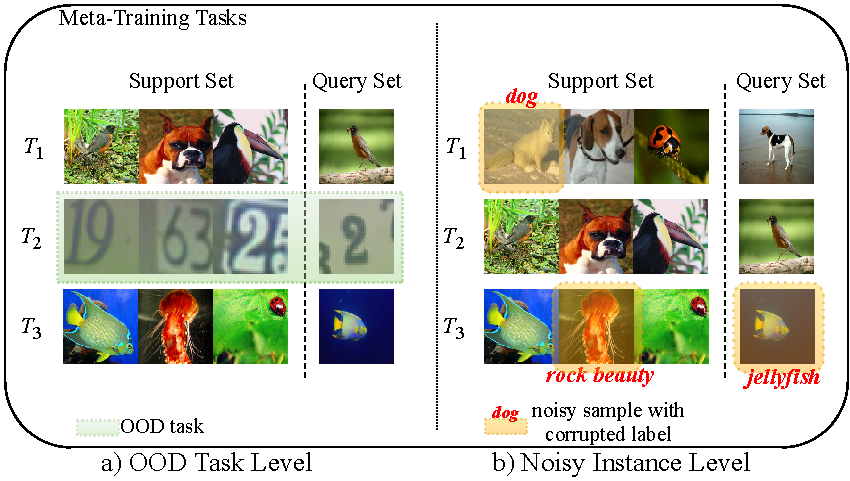
\includegraphics[width=0.47\textwidth, height=4.2cm]{figs/outliers.pdf}
    \vspace{-7mm}
    \caption{We consider corrupted training set for few-shot learning in this work: a) OOD task level and b) noisy instance level. $T_2$ in a) is an OOD task that is sampled from a different distribution. b) contains some noisy samples which are mislabeled. For example, the actual label of the first sample in $T_1$ should be ``\textit{Arctic fox}" which is labeled as ``\textit{dog}"; The labels of two noisy samples in $T_3$ are flipped wrongly. The first one should be ``\textit{rock beauty}," and the other one should be ``\textit{jellyfish}."}
    % {Solid green squares and circles represent tasks sampled from the in-distribution dataset (\textit{e.g.,} \textit{mini}-ImageNet~\citep{ravi2016optimization}); red triangles indicate tasks sampled from out-of-distribution (OOD) dataset (\textit{e.g.,} SVHN~\citep{netzer2011reading}). Training and testing domains (a) are subsets of the data domain; (b) have some overlap between each other where some OOD tasks (\textit{e.g.} $30\%$, etc.) are involved in the training domain; \textbf{We consider type (b) in our paper}.}
    \label{fig:motivation}
\vspace{-8mm}
\end{figure}

\begin{figure*}[!htbp]
%\captionsetup[subfigure]{aboveskip=-2pt,belowskip=-2pt}
    \centering
    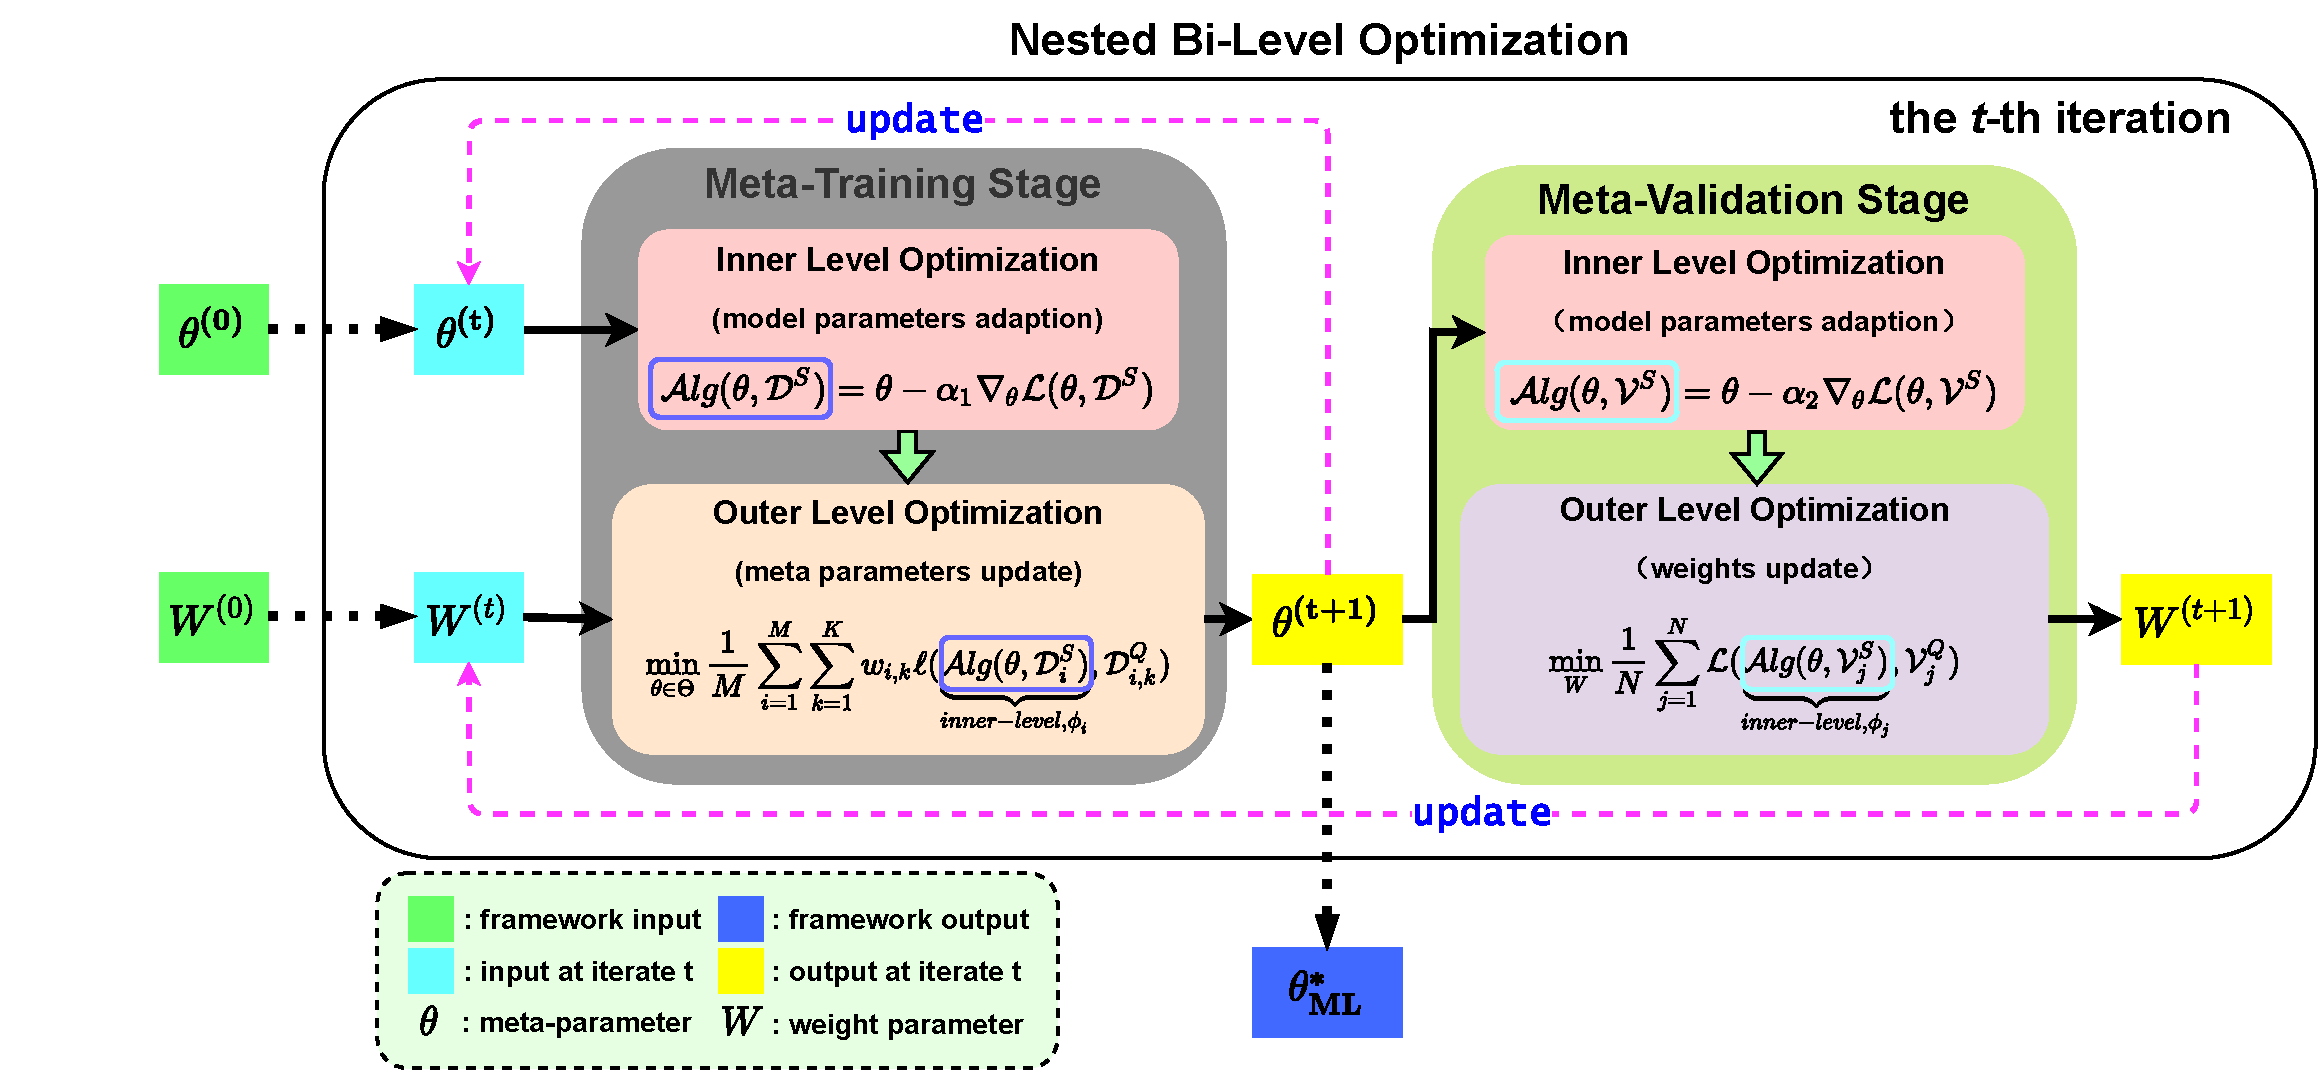
\includegraphics[width=0.85\linewidth, height=6.5cm]{figs/overview.pdf}
    \caption{Overview of our \sysname{} framework that solves a \textit{\biopt{}} optimization problem. (a) In the meta-training stage, model parameters $\phi_i$ of each task are adapted from meta-parameter $\boldsymbol{\theta}$ through the inner level optimization; (b) In the outer-level of the meta-training stage, we update the meta-parameters using the weights $W$ from the previous iterate; (c) Weights are further updated in the meta-validation stage using the gradient of the meta-losses with respect to current $W$.} 
    \label{fig:overview}
    \vspace{-4mm}
\end{figure*}

We motivate the importance of robust meta-learning when meta-training tasks have OOD tasks using the following examples. For example, consider the task of detecting vehicles at night under different weather conditions. In this case, the meta-test tasks only consist of images of vehicles at night. Since the procurement vehicles driving data at night, covering all critical scenarios is difficult, we need a model that can quickly adapt to rare driving conditions. Hence, we consider meta-training tasks to consist of images of the vehicles in multiple lighting scenarios. In this case, some of the tasks in meta-training may degrade the meta-test performance. So, it is vital to have a meta-learning model that is robust to OODs.

Another example is rare lung cancer detection from medical x-ray images. Since the procurement of rare lung cancer images is both problematic and expensive, it is beneficial to use prior knowledge of cancer images. Specifically, the meta-test tasks contain images of rare lung cancer, whereas meta-training tasks consist of general cancer x-ray images. In the examples given above, meta-test tasks belong to specialized slices where the data availability is meager compared to meta-training tasks. The meta-training task distribution is biased compared to that in the meta-test. To keep the whole meta-training tasks for generalization and reduce the adverse impact of the biased distribution in meta-training, we propose a novel robust few-shot learning algorithm in the presence of outliers in meta-training time, which is similar to the corruptions in training time in the traditional robust learning~\citep{schneider2020improving}. This is different from the existing robust few-shot learning papers~\cite{yin2018adversarial, lu2020robust, goldblum2020adversarially} which consider the corruption only happens in meta-test time.     

To simulate the corruptions in meta-training, two levels of outliers (Figure \ref{fig:motivation}) are considered: {\textit{a}}) Out-Of-Distribution (OOD) task, where the meta-training has tasks that are out of distribution to the meta-test tasks (i.e., the meta-test dataset is a specialized slice of meta-train) and {\textit{b}}) noisy instance level, where some of the labels might be noisy (due to human labeling errors or inherent ambiguity of certain classification problems) for meta-training samples. 

A natural way of dealing with corrupted data in meta-training is by assigning weights to either tasks or individual instances. For example, assigning zero weight to OOD or noisy tasks/instances in the meta-train set improves the meta-learning algorithm's performance. Inspired by~\citep{ren2018learning}, in this work, we propose an end-to-end robust meta-learning framework called \sysname{} that can achieve the reweighting schema along with learning good model initialization parameters in the few-shot learning scenario.  

% The resulting problem is an extension of meta-learning called \emph{weighted meta-learning}. Weighted meta-learning has been studied in~\citet{cai2020weightedmeta}, where they study the weighting on a restricted class of loss functions like the square loss and hinge loss. 


%An efficient meta-learning algorithm should learn the corresponding meta-knowledge of vehicle detection or tumor detection useful for faster learning of specialized tasks like detecting vehicles at night or rare cancer.

% \vspace{-1ex}
% \subsection{Our Contributions}
% Our work's significant contribution is introducing the nested MAML (\sysname{}) algorithm, an end-to-end framework for the reweighted MAML training. 

\sysname{} considers the weights as hyper-parameters and uses a small set of meta-validation tasks representing the meta-test tasks to find the optimal hyper-parameters by minimizing the meta-loss on the validation tasks in a \textbf{\biopt{}} manner.  An overview of \sysname{} is given in Figure \ref{fig:overview}. In practice, the size of the meta-validation tasks set required by \sysname{} is tiny compared to the meta-training dataset. Hence, creating a  small and clean meta-validation set is neither expensive nor unrealistic, even for rare specialized use cases of a real-life scenario. A similar strategy has been applied in ~\citep{ren2018learning,shu2019meta,killamsetty2020glister}. However, they focus on traditional supervised learning, and we generalize this to task- and instance-level in a meta-learning setting. Since \sysname{} uses an online framework to perform a joint optimization of the weight hyper-parameters and model parameters for the weighted MAML model, the computational time of ours is comparable to MAML.
% specifically 1.5 times MAML's running time. %Finally, we compare \sysname{}'s performance to existing robust meta-learning and hyperparameter optimization algorithms through extensive experiments on real-world and synthetic datasets for {\textcolor{red}{out-of-distribution (OOD), noisy-labels settings in training data}}.

\noindent \textbf{Contributions of our work are summarized as follows:} 1) We study the general form of the task and instance weighted meta-learning, where we learn the optimal weights and model initialization parameters by optimizing a \textit{\biopt{}} objective function. To the best of our knowledge, ours is the first work that studies the \textit{\biopt{}} optimization problem, which comes naturally in such a new setting. 2) We introduce a novel algorithmic framework \sysname{} that uses a small set of validation tasks to enable robust meta-learning. We solve the \emph{\biopt{}} optimization problem efficiently through a series of practical approximations and provide a theoretical convergence analysis for \sysname{}. In particular, we show that \sysname{} converges in $\mathcal{O}(1/\epsilon^2)$ iterations under reasonable assumptions and contrast this with existing bounds of MAML. 3) We provide comprehensive synthetic and real-world data experiments demonstrating that \sysname{} achieves state-of-the-art results in two scenarios (OOD tasks and noisy instance labels).

\vspace{-1ex}
\section{Related Work}
% \textbf{Meta Learning.} 
% \vspace{-1ex}
There are several lines of meta-learning algorithms: nearest neighbors-based methods~\citep{vinyals2016matching}, recurrent network-based methods~\citep{ravi2016optimization}, and gradient-based methods. As the representative of gradient-based meta-learning algorithms, MAML~\citep{finn2017model} and its variants ~\citep{finn2018probabilistic, nichol2018first, rusu2018meta,rajeswaran2019meta, behl2019alpha, raghu2019rapid, zhao2020fair, zhou2020meta} learn a shared initialization of model parameters across a variety of tasks during the meta-training phase that can adapt to new tasks using a few gradient steps.~\citet{cai2020weightedmeta} proposes a simple weighted meta-learning approach only for the basis regression problem that selects weights by minimizing a data-dependent bound involving an empirical integral probability metric between the weighted sources and target risks. However, this approach cannot be easily extended to complex scenarios with arbitrary loss functions.
% In contrast, \sysname{} can handle arbitrary loss functions.
% and \textit{b}) jointly learn the weights along with the meta-learning model parameters.  % Our \sysname{} algorithm poses the weights as hyper-parameters of the model and tries to estimate these weights by minimizing the nested loss over the model parameters and weight hyper-parameters. \sysname{} can be applied to any loss functions at the expense of the computational costs due to the need for higher-order differentiation in the computation graph.
% ~\cite{yao2020automated} proposes ARML, which extracts the cross-task relations and constructs the meta-knowledge graph to enable the model to find a specific meta learner for the new task.

% \noindent \textbf{Learning with OOD tasks.} %Because of task homogeneity assumption limitation, MAML does not perform well on the training tasks sampled from different distributions ~\citep{vuorio2019multimodal}. 
There are few meta-learning papers discussing learning with OOD tasks. ~\citet{jeong2020ood} propose an OOD detection framework in meta-learning through generating fake samples which resemble in-distribution samples and combine them with real samples. However, they assume the outlier instances exist in the query set, which is different from ours. The most relevant field is from the perspective of task heterogeneity~\citep{vuorio2019multimodal, triantafillou2019meta,yao2020automated}. ~\citet{vuorio2019multimodal} proposed  MMAML to deal with multimodal task distribution with disjoint and far apart modes and generates a set of separate meta-learned prior parameters to deal with each mode of a multimodal distribution. If we view that all the OOD tasks belong to a single mode, this is relevant to our setting. To tackle the distribution drift from meta-training to meta-test, B-TAML~\citep{lee2020l2b} learn to relocate the initial parameters to a new start point based on the arriving unseen tasks in the meta-test. The setting considered in our work and B-TAML work can be viewed as similar if we assume some of the datasets considered in the multi-dataset classification setting of B-TAML as OOD datasets.
%Among the meta-training tasks, some tasks are Out-of-Distribution (OOD) if they have a very different distribution from others. 

% \noindent \textbf{Learning with noisy labels.} 
To tackle samples with corrupted labels, some researches~\citep{luo2015foveation, jalal2017robust, wang2019direct} introduce noise-robust models.~\citet{ren2018learning} and~\citet{shu2019meta} propose a noisy data filtering strategy using an instance reweighting strategy where the weights are learned automatically. However, the effect of noisy labels on few-shot learning requires more attention. Although ~\citep{yin2018adversarial,lu2020robust,goldblum2020adversarially} proposes robust meta-learning or few-shot learning, they assume a presence of outliers containing in meta-test, which is different from ours. 
% In contrast, \sysname{} does not require any additional information about noisy samples in its learning.}%to deal with the training tasks containing data instances with noisy labels. 

% In contrast, ~\citep{han2018co, chen2019understanding}propose noisy data filtering techniques to reduce noisy labels' impact. 
%Our paper is the first to consider the training tasks with noisy labels without any additional information about noisy samples in the few-shot learning framework to the best of our knowledge. 

%for noise filtering that solves a bi-level optimization problem on instance weights. In contrast~\cite{shu2019meta} uses an MLP as a weighting function, explicitly mapping sample weights adaptively from the data. 
%Many researchers focus on learning with noisy labels to avoid extravagant relabeling costs by improving deep learning models' robustness.
% ~\cite{han2018co} proposes a co-teaching model that trains two neural networks simultaneously, and they will teach each other to detect noisy samples. INCV~\citep{chen2019understanding} applies cross-validation to randomly split noisy datasets and use the selected samples to train the model. ~\cite{ren2018learning} proposes a gradient-based method to assign weights to training samples by online meta-learning strategy.
% For comparison, we consider two baselines that use Co-teaching~\citep{han2018co} and INCV~\citep{chen2019understanding} to clean noisy datasets first and apply MAML to the selected data.

\section{Preliminaries}
\subsection{Notations}
In the setting of meta-learning for few-shot learning, there is a set of meta-training tasks $\{\mathcal{T}_i\}_{i=1}^M$ sampled from the probability distribution 
$p_{tr}(\mathcal{T})$. Each few-shot learning task $\mathcal{T}_i$ has an associated dataset $\mathcal{D}_i$ containing two disjoint sets $\{\mathcal{D}^{S}_{i},\mathcal{D}^{Q}_{i}\}$, where the superscripts $S$ and $Q$ denote support set and query set respectively. The query sets take the form $\mathcal{D}^{Q}_{i} = \{\boldsymbol{x}_i^k, {y}_i^k\}_{k=1}^K$ and similarly for $\mathcal{D}^{S}_{i}$. Meta-validation tasks are denoted in a similar manner: $\{\mathcal{T}^{\mathcal{V}}_{j}= \{\mathcal{V}_{j}^{S}, \mathcal{V}_{j}^{Q}\} \}_{j = 1} ^ {N}$
% We are interested in learning the models of the form $h : \mathcal{X}\mapsto\mathcal{Y}$.  
Let the loss function be denoted as $\mathcal{L}(\boldsymbol{\phi}, \mathcal{D})$ with $\boldsymbol{\phi}$  denoting model parameters and $\mathcal{D}$ denoting the dataset, and $\ell(\boldsymbol{\theta}, d)$ with model parameters $\boldsymbol{\theta}$ on the data-point $d$. For example, $\mathcal{L}(\phi, \mathcal{D}_i^{Q})$ denotes the loss of the $i^{th}$ training task query set $\mathcal{D}_i^{Q}$ for given model parameters $\phi \in \boldsymbol{\Phi}\equiv \mathbb{R}^d$, where $\boldsymbol{\phi}:=\mathcal{A}lg(\boldsymbol{\theta}, \mathcal{D}^S)$ and $\boldsymbol{\theta}\in \boldsymbol{\Theta} \equiv \mathbb{R}^d$ is the meta-parameter. $\mathcal{A}lg(\cdot)$ corresponds to a learning algorithm.
% The functional form of $\mathcal{A}lg(\cdot)$ for a single gradient step is given section 3.2.

% We weigh each datapoint (instance) in the query set of task $\mathcal{T}_i$ with a weight $w_{ik}\in \mathbb{R}$, where $k=1,...,K$ denotes the datapoint index. 
% Instance weights are optimized using a held-out set of meta-validation tasks $\{\mathcal{T}_j ^{\mathcal{V}}\}_{j=1}^N$ drawn from $p_{val}(\mathcal{T})$. Similar to meta-training tasks, each task $\mathcal{T}^{\mathcal{V}}_j$ in the meta-validation set contains a support set $\mathcal{V}_j^S$ and a query set $\mathcal{V}_j^Q$. 
% Let $\ell(\boldsymbol{\theta}, d)$ be the loss on the query data-point $d$ corresponding to model parameters $\boldsymbol{\theta}$. 

For notation convenience, we write $\mathcal{L}_i(\phi) := \mathcal{L}(\phi, \mathcal{D}_i^{Q})$; $\mathcal{L}_{V_j}(\phi):=\mathcal{L}(\phi, \mathcal{V}_j^{Q})$;  $\widehat{\mathcal{L}}_{V_j}(\boldsymbol{\phi}) := \mathcal{L}(\boldsymbol{\phi}, \mathcal{V}_j^{S})$. We denote scalars by lower case italic letters, vectors by lower case boldface letters, and matrices by capital italic letters throughout the paper. A table of notations with corresponding explanations is given in Appendix~\ref{app:notations}.

% For notation convenience we introduce the following terms. Let $\mathcal{L}_i(\phi) := \mathcal{L}(\phi, \mathcal{D}_i^{Q})$ where $\mathcal{L}_i(\phi)$ is the loss of the $i^{th}$ training task query set $\mathcal{D}_i^{Q}$ for given model parameters $\phi$. Let $\mathcal{L}_{V_j}(\phi):=\mathcal{L}(\phi, \mathcal{V}_j^{Q})$ where $\mathcal{L}_{V_j}(\phi)$ is the loss of the $j^{th}$ validation task query set $\mathcal{V}_j^{Q}$ for given model parameters $\phi$. Let $\widehat{\mathcal{L}}_{V_j}(\boldsymbol{\phi}) := \mathcal{L}(\boldsymbol{\phi}, \mathcal{V}_j^{S})$ where $\widehat{\mathcal{L}}_{V_j}(\phi)$ is the loss calculated on the $j^{th}$ validation task support set $\mathcal{V}_j^{S}$ for given model parameters $\phi$.

% The goal for task $\mathcal{T}_i$ is to learn the model-specific parameter $\phi_i$ using support set $\mathcal{D}_{i}^{S}$ such that we can minimize the query set loss $\mathcal{L}(\phi_i, \mathcal{D}_{i}^{Q})$.

\subsection{Model-Agnostic Meta-Learning}
The goal of MAML~\cite{finn2017model} is to obtain the optimal initial parameters that minimize the meta-training objective:
\begin{equation}
\begin{aligned}
    \label{meta-objective}
    \overbrace{\boldsymbol{\theta}^*_{ML}= \argmin_{\boldsymbol{\theta} \in \boldsymbol{\Theta}}{\mathcal{F}(\boldsymbol{\theta})}}^{outer-level}\text{\hspace{1.7cm}}\\
    \text{where, }\mathcal{F}(\boldsymbol{\theta}) = \frac{1}{M}\sum\nolimits_{i=1}^{M}\mathcal{L}(\overbrace{\mathcal{A}lg(\boldsymbol{\theta}, \mathcal{D}_{i}^{S})}^{inner-level}, \mathcal{D}_{i}^{Q})\text{\hspace{0.5cm}}
\end{aligned}
\end{equation}
This is a bi-level optimization problem, where we construe that $\mathcal{A}lg(\boldsymbol{\theta}, \mathcal{D}_{i}^{S})$ explicitly or implicitly optimizes the inner-level task-specific adaptation. The outer-level corresponds to the meta-training objective of generalizing well (i.e. low test error) on the query set of each task after adaptation. 
 
Since $\mathcal{A}lg(\boldsymbol{\theta}, \mathcal{D}_{i}^{S})$ corresponds to single or multiple gradient descent steps. In case of a single gradient descent, $\mathcal{A}lg(\boldsymbol{\theta}, \mathcal{D}_{i}^{S})$ can be perceived as follwing:
\begin{equation}
\label{param-adaptation}  \mathcal{A}lg(\boldsymbol{\theta}, \mathcal{D}_{i}^{S}) = \boldsymbol{\theta} - \alpha \nabla_{\boldsymbol{\theta}}\mathcal{L}(\boldsymbol{\theta}, \mathcal{D}_{i}^{S})
\end{equation}
where $\alpha $ is a learning rate.
% hyper-parameter, which is a scalar or can also be a vector ~\citep{li2017meta}. 
% Works like ~\cite{behl2019alpha} show an online learning rate hyper-parameter $\alpha$ adaptation method that removes the need for fine-tuning it. 
As shown above, the meta-training objective assumes equal weights to each task for generalization, which may not be ideal in the case of adversaries in the training tasks set.

\section{Methodology}
%%
%% This is file `algorithm.sty',
%% generated with the docstrip utility.
%%
%% The original source files were:
%%
%% algorithms.dtx  (with options: `algorithm')
%% This is a generated file.
%% 
%% Copyright (C) 1994-2004   Peter Williams <pwil3058@bigpond.net.au>
%% Copyright (C) 2005-2009   Rogério Brito <rbrito@ime.usp.br>
%% 
%% This document file is free software; you can redistribute it and/or
%% modify it under the terms of the GNU Lesser General Public License as
%% published by the Free Software Foundation; either version 2 of the
%% License, or (at your option) any later version.
%% 
%% This document file is distributed in the hope that it will be useful, but
%% WITHOUT ANY WARRANTY; without even the implied warranty of
%% MERCHANTABILITY or FITNESS FOR A PARTICULAR PURPOSE.  See the GNU Lesser
%% General Public License for more details.
%% 
%% You should have received a copy of the GNU Lesser General Public License
%% along with this document file; if not, write to the Free Software
%% Foundation, Inc., 59 Temple Place - Suite 330, Boston, MA 02111-1307,
%% USA.
%% 
\NeedsTeXFormat{LaTeX2e}[1999/12/01]
\ProvidesPackage{algorithm}
   [2009/08/24 v0.1 Document Style `algorithm' - floating environment]
\RequirePackage{float}
\RequirePackage{ifthen}
\newcommand{\ALG@within}{nothing}
\newboolean{ALG@within}
\setboolean{ALG@within}{false}
\newcommand{\ALG@floatstyle}{ruled}
\newcommand{\ALG@name}{Algorithm}
\newcommand{\listalgorithmname}{List of \ALG@name s}
% Declare Options:
% * first: appearance
\DeclareOption{plain}{
  \renewcommand{\ALG@floatstyle}{plain}
}
\DeclareOption{ruled}{
  \renewcommand{\ALG@floatstyle}{ruled}
}
\DeclareOption{boxed}{
  \renewcommand{\ALG@floatstyle}{boxed}
}
% * then: numbering convention
\DeclareOption{part}{
  \renewcommand{\ALG@within}{part}
  \setboolean{ALG@within}{true}
}
\DeclareOption{chapter}{
  \renewcommand{\ALG@within}{chapter}
  \setboolean{ALG@within}{true}
}
\DeclareOption{section}{
  \renewcommand{\ALG@within}{section}
  \setboolean{ALG@within}{true}
}
\DeclareOption{subsection}{
  \renewcommand{\ALG@within}{subsection}
  \setboolean{ALG@within}{true}
}
\DeclareOption{subsubsection}{
  \renewcommand{\ALG@within}{subsubsection}
  \setboolean{ALG@within}{true}
}
\DeclareOption{nothing}{
  \renewcommand{\ALG@within}{nothing}
  \setboolean{ALG@within}{true}
}
\DeclareOption*{\edef\ALG@name{\CurrentOption}}
% ALGORITHM
%
\ProcessOptions
\floatstyle{\ALG@floatstyle}
\ifthenelse{\boolean{ALG@within}}{
  \ifthenelse{\equal{\ALG@within}{part}}
     {\newfloat{algorithm}{htbp}{loa}[part]}{}
  \ifthenelse{\equal{\ALG@within}{chapter}}
     {\newfloat{algorithm}{htbp}{loa}[chapter]}{}
  \ifthenelse{\equal{\ALG@within}{section}}
     {\newfloat{algorithm}{htbp}{loa}[section]}{}
  \ifthenelse{\equal{\ALG@within}{subsection}}
     {\newfloat{algorithm}{htbp}{loa}[subsection]}{}
  \ifthenelse{\equal{\ALG@within}{subsubsection}}
     {\newfloat{algorithm}{htbp}{loa}[subsubsection]}{}
  \ifthenelse{\equal{\ALG@within}{nothing}}
     {\newfloat{algorithm}{htbp}{loa}}{}
}{
  \newfloat{algorithm}{htbp}{loa}
}
\floatname{algorithm}{\ALG@name}
\newcommand{\listofalgorithms}{\listof{algorithm}{\listalgorithmname}}
\endinput
%%
%% End of file `algorithm.sty'.


\section{Experiments}

\section{Experiments}
\label{sec:experiment}

\begin{table}[t]
\centering
\small
\resizebox{0.99\linewidth}{!}{
\begin{tabular}{lcccc}
\multirow{2}{1.5cm}{\textbf{Methods}} & \multicolumn{2}{c}{\textbf{Far-OOD}} & \multicolumn{2}{c}{\textbf{Near-OOD}}\\
\cmidrule{2-5}
& \textbf{FPR95}  & \textbf{AUROC} & \textbf{FPR95}  & \textbf{AUROC}\\
& $\downarrow$ & $\uparrow$ & $\downarrow$ & $\uparrow$ \\
\toprule
\emph{Using model outputs}\\
MSP~\cite{hendrycks2016baseline} & 52.11 & 91.79 & 64.66 & 85.28 \\
ODIN~\cite{liang2018enhancing}  & 26.47 & 94.48 & 52.32 & 88.90\\
GODIN~\cite{hsu2020generalized}  & 17.42  & 95.84 & 60.69 & 82.37 \\
Energy score~\cite{liu2020energy}  & 28.40 & 94.22 & 50.64 & 88.66 \\
ReAct~\cite{sun2021react} & 33.12 & 94.32 & 53.51 & 88.96\\
GradNorm~\cite{huang2021importance} & 24.79 & 92.58 & 65.44 & 79.31\\
LogitNorm~\cite{wei2022mitigating}  & 19.61 & 95.51 & 55.08 & 88.03\\
DICE~\cite{sun2022dice}  & 20.83 & 95.24 & 58.60 & 87.11 \\
\midrule
\emph{Using feature representations}\\
Mahalanobis~\cite{lee2018simple} & 44.55 & 82.56 & 87.71 & 78.93 \\
KNN~\cite{sun2022knn}  & 18.50 & 96.36 & 58.34 & 87.90 \\
\midrule 
 \name (ours) & \textbf{14.99} & \textbf{97.15}  & \textbf{50.10} &  \textbf{89.80}\\
 & $\pm{0.87}$ & $\pm{0.27}$ & $\pm{1.09}$ & $\pm{0.65}$\\
\bottomrule
\end{tabular}}
\caption{\small Performance comparison on near-OOD and far-OOD detection task. Architecture used is DenseNet-101 and ID data is CIFAR-10. We report the mean and variance across 3 training runs.}
\label{tab:hard_ood}
\end{table}
\begin{table}[t]
\small
\centering
\resizebox{0.99\linewidth}{!}{
\begin{tabular}{lccc}
\textbf{Method} & \textbf{FPR95}  & \textbf{AUROC} & \textbf{ID Acc.}\\
& $\downarrow$ & $\uparrow$ & $\uparrow$ \\
\toprule
\emph{Methods using model outputs}\\
MSP~\cite{hendrycks2016baseline} & 77.59 & 76.47 &  75.14\\
ODIN~\cite{liang2018enhancing} & 56.39 & 86.02 & 75.14\\
GODIN~\cite{hsu2020generalized} & 44.08 &  89.05 & 74.37\\
Energy score~\cite{liu2020energy} & 57.07 &  84.83 &  75.14\\
ReAct~\cite{sun2021react} & 75.06 & 79.51 & 66.56\\
GradNorm~\cite{huang2021importance} & 63.05 & 79.80 & 75.14\\
LogitNorm~\cite{wei2022mitigating} & 61.10 & 84.72 & 75.42\\
DICE~\cite{sun2022dice} & 49.72 & 87.23 & 68.65 \\
\midrule 
\emph{Methods using feature representations}\\
Mahalanobis~\cite{lee2018simple} & 56.93 & 80.27 &  75.14\\
KNN~\cite{sun2022knn} & 47.21 & 85.27 & 75.14\\
\midrule 
 \name (ours) & \textbf{31.25} & \textbf{90.76} & \textbf{75.59}\\
& $\pm{1.25}$ & $\pm{0.36}$ & $\pm{0.08}$\\
\bottomrule
\end{tabular}}
\caption{\small Performance comparison on CIFAR-100 dataset. We use DenseNet-101 for all baselines. Best  results are in \textbf{bold}. We report the mean and variance across 3 different training runs.}
\label{tab:cifar-100}
\end{table}
In this section, we extensively evaluate the effectiveness of our proposed method. 
The goal of our experimental sections is to mainly answer the following questions: (1) Can \name alleviate the curse of dimensionality? (2) How does \name compare against the state-of-the-art OOD detection methods?  Due to space constraints, extensive experimental details are in Appendix C. Our code is open-sourced for the research community.


\subsection{Evaluation on Common Benchmarks}
\label{subsec:common_benchmark}

\noindent \textbf{Datasets.} In this section, we make use of commonly studied CIFAR-10 (10 classes) and CIFAR-100 (100 classes)~\cite{krizhevsky2009learning} datasets as ID. Both datasets consist of images of size $32 \times 32$. We use the standard split with $50,000$ images for training and $10,000$ images for testing. We evaluate the methods on common OOD datasets: \texttt{Textures}~\cite{cimpoi2014describing}, \texttt{SVHN}~\cite{svhn}, \texttt{LSUN-Crop}~\cite{yu2015lsun}, \texttt{LSUN-Resize}~\cite{yu2015lsun}, \texttt{iSUN}~\cite{xu2015turkergaze}, and \texttt{Places365}~\cite{zhou2017places}. Images in all these test datasets are of size $32 \times 32$. 


\paragraph{Evaluation metrics.} We compare the performance of various methods using the following metrics: 
(1) {FPR95} measures the false positive rate (FPR) of OOD samples when $95\%$ of ID samples are correctly classified;
(2) {AUROC} is the area under the Receiver Operating Characteristic curve; 
and (3) {ID Acc.} measures the ID classification accuracy.

\vspace{0.2cm}
\noindent \textbf{Comparison with competitive methods.} In Table~\ref{tab:cifar-100}, we provide a comprehensive comparison with competitive OOD detection baselines on  CIFAR-100. {We provide a detailed description of baseline approaches in Appendix C.3.} We observe that our proposed method \name significantly outperforms the latest rivals. For a fair comparison, we divide the baselines into two categories: methods using model outputs and methods using feature representations.
From Table~\ref{tab:cifar-100}, we highlight two salient observations: (1) Considering methods based on feature representations, \name outperforms KNN (non-parametric) and Mahalanobis (parametric) by \textbf{15.96\%} and \textbf{25.68\%} respectively in terms on FPR95. The results validate that learning feature subspace effectively alleviates the ``curse-of-dimensionality" problem that is troubling the existing KNN approach. (2) Further, \name also performs better than output-based methods such as ReAct~\cite{sun2021react}. Specifically, with CIFAR-100 as ID, \name provides a $\mathbf{43.81}\%$ improvement in FPR95 as compared to ReAct~\cite{sun2021react}. Notably, \name provides a \textbf{18.47\%} improvement compared to~\cite{sun2022dice}, a post-hoc sparsification method. While DICE can severely affect the ID test accuracy (68.65\%), \name exhibits stronger classification performance (75.59\%) by baking in the inductive bias of subspaces through training. An extensive discussion is provided in Section~\ref{sec:discussion}. 



\paragraph{Evaluation on near-OOD data.} In Table~\ref{tab:hard_ood}, we compare the performance in detecting near-OOD data, which refers to samples near the ID data. Near-OOD is particularly challenging to detect, and can often be misclassified as ID. We report the performance on CIFAR-10 (ID) vs. CIFAR-100 (OOD), which is the most commonly used dataset pair for this task. We observe that \name consistently outperforms existing algorithms for near-OOD detection tasks, further demonstrating its strengths. Compared to KNN, \name reduces the FPR95 by 8.24\%. For completeness, we also provide far-OOD evaluation results on CIFAR-10, where \name achieves an average FPR95 of 14.99\%. Full result on each test dataset for CIFAR-10 is available in Appendix D.4.



\begin{table}[t]
\small
\centering
\resizebox{0.95\linewidth}{!}{
\begin{tabular}{lccc}
\textbf{Method} & \textbf{Dataset (ID)} & \textbf{FPR95}  & \textbf{AUROC} \\
& & $\downarrow$ & $\uparrow$  \\
\toprule
Mahalanobis~\cite{lee2018simple} & CIFAR-10 & 44.55 & 82.56  \\

\name (w. Mahalanobis) & CIFAR-10 &  \textbf{34.68} &  \textbf{87.87} \\
\midrule
Mahalanobis~\cite{lee2018simple} & CIFAR-100 & 56.93 & 80.27  \\

\name (w. Mahalanobis) & CIFAR-100 &  \textbf{55.05} &  \textbf{80.77} \\
\bottomrule
\end{tabular}}
\caption{\small \name is also compatible with parametric approaches such as Mahalanobis distance~\cite{lee2018simple}. The model is DenseNet. All values are averaged over six OOD test datasets.}
\label{tab:compatibility}
\end{table}


\paragraph{Compatibility with other distance-based approaches.} 

Beyond KNN~\cite{sun2022knn}, the Mahalanobis distances~\cite{lee2018simple} is also one of the most popular distance-based approaches to detect OOD. 
However, all prior solutions measure the distance with a full feature space which can also suffer from the curse of dimensionality. 
In this section, we show that subspace learning can also benefit parametric approaches like Mahalanobis distance~\cite{lee2018simple}. In Table~\ref{tab:compatibility}, we compare the OOD detection performance of using Mahalanobis distance on the vanilla model and the model trained with \name. 
We see that coupling subspace learning (in training) with Mahalanobis distance (in testing) reduces FPR95 by {9.87\%} and {1.88\%} on CIFAR-10 and CIFAR-100 datasets respectively.

\begin{table}[t]
\small
\centering
\resizebox{0.55\linewidth}{!}{
\begin{tabular}{lcc}
\toprule
\multirow{2}{2cm}{\textbf{Training Method}} &  CIFAR-10 & CIFAR-100 \\ 
& \multicolumn{2}{c}{(Train time in hours)} \\
\midrule
Standard & $2.10$ & $2.25$\\ 
 \name & $1.75$ & $1.89$ \\
\bottomrule
\end{tabular}}
\caption{\small \textbf{Computational cost for training}. trained using ResNet-101. 
Model used is DenseNet-101. For the comparison, we used the software configuration as reported in Appendix C.2.}
\label{tab:train_time}
\end{table}
% 
\paragraph{Computational complexity.}  In Table~\ref{tab:train_time}, we compare the training time of \name with the standard training method using cross-entropy loss. We observe that training using \name incurs no additional computation overhead but rather is slightly more efficient compared to standard training procedures. This is because we perform gradient descent only on a subset of weights corresponding to the selected feature subspace. Thus, our method overall leads to faster updates and convergence. {In Appendix D.1, we further show that
\name remains competitive and outperforms the KNN counterpart on other common architecture.}

\section{Conclusion}
\section{Conclusion}
In this paper, we introduced a new ad-hoc retrieval approach GRMM which explicitly incorporates document-level word relationships into the matching function. The flexible graph structure allows the model to find more comprehensive matching patterns and less noises. GRMM exceedingly advances the performance over various baselines, where it empirically witnesses an increment by a large margin on longer documents. Further studies exhibited the rationality and effectiveness of GRMM. There are also possible extensions, such as training with large click logs \cite{jiang2016learning} and query descriptions. Another interesting future work is to extend the current graph with lexical or knowledge graphs which might contain more useful information. 

\bibliography{main}

\bigskip
\appendix
% %File: formatting-instruction.tex
% \documentclass[letterpaper]{article} % DO NOT CHANGE THIS
% \usepackage{aaai24}  % DO NOT CHANGE THIS
% \usepackage{times}  % DO NOT CHANGE THIS
% \usepackage{helvet}  % DO NOT CHANGE THIS
% \usepackage{courier}  % DO NOT CHANGE THIS
% \usepackage[hyphens]{url}  % DO NOT CHANGE THIS
% \usepackage{graphicx} % DO NOT CHANGE THIS
% \urlstyle{rm} % DO NOT CHANGE THIS
% \def\UrlFont{\rm}  % DO NOT CHANGE THIS
% \usepackage{natbib}  % DO NOT CHANGE THIS AND DO NOT ADD ANY OPTIONS TO IT
% \usepackage{caption} % DO NOT CHANGE THIS AND DO NOT ADD ANY OPTIONS TO IT
% \frenchspacing  % DO NOT CHANGE THIS
% \setlength{\pdfpagewidth}{8.5in}  % DO NOT CHANGE THIS
% \setlength{\pdfpageheight}{11in}  % DO NOT CHANGE THIS
% \usepackage{algorithm}
% % \usepackage{algorithmic}
% \usepackage{multirow}
% \usepackage{makecell}
% \usepackage{pifont}
% \usepackage{bbding}
% \usepackage{amsmath}
% \usepackage{amssymb}
% \usepackage{algpseudocode}
% \usepackage{booktabs}
% \usepackage{amstext}
% \usepackage{bm}
% \usepackage{subfigure}
% \newcommand{\eg}{\textit{e}.\textit{g}.}
% \usepackage{enumitem}
% \usepackage[table]{xcolor}

% \usepackage{url}            % simple URL typesetting
% \usepackage{booktabs}       % professional-quality tables
% \usepackage{mathtools,amssymb}
% \usepackage{amsfonts}       % blackboard math symbols
% \usepackage{nicefrac}       % compact symbols for 1/2, etc.
% \usepackage{microtype}      % microtypography
% \usepackage{pgfplots,pgfplotstable}
% \pgfplotsset{compat=1.14}
% \usepackage{array,colortbl}
% \usepackage{xcolor}
% \usepackage{algorithm,algorithmicx,algpseudocode}
% \usepackage[capitalise]{cleveref}
% \usepackage{caption}
% \usepackage{graphbox}
% \usepackage{placeins}
% % \usepackage{wrapfig}
% \usepackage{subcaption}
% \usepackage{etoolbox}

% \newcommand{\bzero}{\mathbf{0}}
% \newcommand{\bone}{\mathbf{1}}
% \newcommand{\bb}{\mathbf{b}}
% \newcommand{\bu}{\mathbf{u}}
% \newcommand{\bv}{\mathbf{v}}
% \newcommand{\bw}{\mathbf{w}}
% \newcommand{\bx}{\mathbf{x}}
% \newcommand{\by}{\mathbf{y}}
% \newcommand{\bz}{\mathbf{z}}
% \newcommand{\bxh}{\hat{\mathbf{x}}}
% \newcommand{\btheta}{{\boldsymbol{\theta}}}
% \newcommand{\bphi}{{\boldsymbol{\phi}}}
% \newcommand{\bepsilon}{{\boldsymbol{\epsilon}}}
% \newcommand{\bmu}{{\boldsymbol{\mu}}}
% \newcommand{\bnu}{{\boldsymbol{\nu}}}
% \newcommand{\bSigma}{{\boldsymbol{\Sigma}}}
% \newcommand{\vardbtilde}[1]{\tilde{\raisebox{0pt}[0.85\height]{$\tilde{#1}$}}}
% \newcommand{\defeq}{\coloneqq}
% \newcommand{\grad}{\nabla}
% \newcommand{\E}{\mathbb{E}}
% \newcommand{\Var}{\mathrm{Var}}
% \newcommand{\Cov}{\mathrm{Cov}}
% \newcommand{\Ea}[1]{\E\left[#1\right]}
% \newcommand{\Eb}[2]{\E_{#1}\!\left[#2\right]}
% \newcommand{\Vara}[1]{\Var\left[#1\right]}
% \newcommand{\Varb}[2]{\Var_{#1}\left[#2\right]}
% \newcommand{\kl}[2]{D_{\mathrm{KL}}\!\left(#1 ~ \| ~ #2\right)}
% \newcommand{\pdata}{{p_\mathrm{data}}}
% \newcommand{\bA}{\mathbf{A}}
% \newcommand{\bI}{\mathbf{I}}
% \newcommand{\bJ}{\mathbf{J}}
% \newcommand{\bH}{\mathbf{H}}
% \newcommand{\bL}{\mathbf{L}}
% \newcommand{\bM}{\mathbf{M}}
% \newcommand{\bQ}{\mathbf{Q}}
% \newcommand{\bR}{\mathbf{R}}

% \begin{document}
\onecolumn
\section{Appendix}

\subsection{Settings of PatchDiff}
The denoising step $T$ of our PatchDiff is $1000$, and the values of images and positional tensors are normalized into a range of $[-1, 1]$. We use AdamW optimizers with a initial learning rate of 1e-3 and a one-cycle learning rate scheduler. The weight decay strength is set to $0.0001$. The global noise $\epsilon_g$ is sampled from a global Gaussian distribution $mathcal{N}_g$ which has a standard deviation of $\sigma_g=0.02$ and every pixel has the identical noise vector. 

To better demonstrate the training and sampling differences between the PatchDiff and DDPM~\cite{DDPM}, we further present the algorithm details 
of training and sampling in Algorithm 1 and Algorithm 2. In particular, $\bepsilon_\theta$ is a function approximator intended to predict $\epsilon_1$ from $\bx_t$, $\epsilon_g$ is the global noise we introduced, and other variables are the same as in DDPM. Actually the sampling process is completely identical to the DDPM and without affected by the introducing of $\epsilon_g$ in the training stage.
\begin{figure}[!htpb]
\begin{minipage}[t]{0.495\textwidth}
\begin{algorithm}[H]
  \caption{Training} \label{alg:training}
  \small
  \begin{algorithmic}[1]
    \Repeat
      \State $\bx_0 \sim q(\bx_0)$
      \State $t \sim \mathrm{Uniform}(\{1, \dotsc, T\})$
      \State $\bepsilon_{1}\sim\mathcal{N}(\mathbf{0}, \mathbf{I}), \bepsilon_{g}\sim\mathcal{N}_g(\mathbf{0}, \sigma_g\mathbf{I})$
      \State Take gradient descent step on
      \State $\grad_\theta \left\| \bepsilon_1 - \bepsilon_\theta\bigl(\sqrt{\bar{\alpha}_t} \mathbf{x}_0 + \sqrt{1-\bar{\alpha}_t} \bepsilon_1 + \bepsilon_g, t\bigr) \right\|^2$
    \Until{converged}
  \end{algorithmic}
\end{algorithm}
\end{minipage}
\hfill
\begin{minipage}[t]{0.495\textwidth}
\begin{algorithm}[H]
  \caption{Sampling} \label{alg:sampling}
  \small
  \begin{algorithmic}[1]
    \vspace{.04in}
    \State $\bx_T \sim \mathcal{N}(\mathbf{0}, \mathbf{I})$
    \For{$t=T, \dotsc, 1$}
      \State $\bz \sim \mathcal{N}(\mathbf{0}, \mathbf{I})$ if $t > 1$, else $\bz = \mathbf{0}$
      \State $\bx_{t-1} = \frac{1}{\sqrt{\alpha_t}}\left( \bx_t - \frac{1-\alpha_t}{\sqrt{1-\bar\alpha_t}} \bepsilon_\theta(\bx_t, t) \right) + \sigma_t \bz$
    \EndFor
    \State \textbf{return} $\bx_0$
    \vspace{.04in}
  \end{algorithmic}
\end{algorithm}
\end{minipage}
% \vspace{-1em}
\end{figure}
% \vspace{0.2cm}

\subsection{Settings of Patch-based Detectors}
\subsubsection{Data augmentation}
We first present the data augmentation details applied during the training of detectors in MVTec AD and MVTec LOCO, as respectively illustrated in Table~\ref{tab:augmentation_mvtec} and Table~\ref{tab:augmentation_loco}, where $p$ denotes the probability of the images being with color jitter. It is worthy note that a larger color jitter range is applied for each generated set, which is expected to be helpful for learning color-level anomalies without training additional generators and detectors. (In principle, GRAD should expose the color-level structures by directly reduce the receptive field size of PatchDiff to 0 and generate pure noise images, then learn the color-level anomalies by level-1 detector)

\begin{table}[!htbp]
\centering
\renewcommand{\arraystretch}{1.}
\footnotesize
\resizebox{0.9\textwidth}{!}{
\begin{tabular}{lccccc}
\toprule
  &  &  &  & \multicolumn{2}{c}{Color jitter ($p=0.2$)} \\
\cmidrule{5-6}
Category  & Vertical flip & Horizontal flip & Random rotation ($\pm5^\circ$) & Normal data & Generated data\\
\midrule
Bottle  & \checkmark & \checkmark & \checkmark & $0.05$ & $0.5$\\
Cable  & \ding{55} & \ding{55} & \checkmark & $0.05$ & $0.5$\\
Capsule  & \ding{55} & \ding{55} & \checkmark &$0.05$ & $0.5$\\
Carpet  & \checkmark & \checkmark & \checkmark &$0.05$ & $0.5$\\
Grid  & \checkmark & \checkmark & \checkmark & $0.05$ & $0.5$\\
Hazelnut  & \checkmark & \checkmark & \checkmark & $0.05$ & $0.5$\\
Leather  & \checkmark & \checkmark & \checkmark & $0.05$ & $0.5$\\
Metal Nut  & \ding{55} & \ding{55} & \checkmark & $0.05$ & $0.5$\\
Pill  & \ding{55} & \ding{55} & \checkmark & $0.05$ & $0.5$\\
Screw  & \checkmark & \checkmark & \checkmark & $0.05$ & $0.5$\\
Tile  & \checkmark & \checkmark & \checkmark & $0.05$ & $0.5$\\
Toothbrush  & \ding{55} & \checkmark & \checkmark & $0.05$ & $0.5$\\
Transistor  & \ding{55} & \checkmark & \checkmark & $0.05$ & $0.5$\\
Wood  & \checkmark & \checkmark & \checkmark & $0.05$ & $0.5$\\
Zipper  & \checkmark & \checkmark & \checkmark & $0.05$ & $0.5$\\
\bottomrule
\end{tabular}}
\caption{Overview of the dataset augmentation techniques applied during training to each of the sub-dataset present in MVTec AD, similar to the setting as relative works~\cite{MVloco}.}
\label{tab:augmentation_mvtec}
\end{table}

\begin{table}[!htbp]
\centering
\footnotesize
\resizebox{1\textwidth}{!}
{
\begin{tabular}{lccccc}
\toprule
  &  &  &  & \multicolumn{2}{c}{Color jitter ($p=0.2$)} \\
\cmidrule{5-6}
Category  & Vertical flip & Horizontal flip & Random rotation ($\pm5^\circ$) & Normal data & Generated data\\
\midrule
Breakfast Box  & \ding{55} & \ding{55} & \checkmark & $0.05$ & $0.5$\\
Screw Bag & \checkmark & \checkmark & \checkmark & $0.05$  & $0.5$\\
Pushpins & \checkmark & \checkmark & \checkmark & $0.05$  & $0.5$\\
Splicing Connectors & \checkmark & \checkmark & \checkmark & $0.05$  & $0.5$\\
Juice Bottle & \ding{55} & \ding{55} & \checkmark & $0.05$  & $0.5$\\
\bottomrule
\end{tabular}}
\caption{Overview of the dataset augmentation techniques applied during training to each of the sub-dataset present in MVTec LOCO, similar to the setting as relative works~\cite{MVloco}.}
\label{tab:augmentation_loco}
\end{table}

\begin{table}[!htpb]
\centering
\footnotesize
\begin{tabular}{lcccc}
\toprule
Dataset     &Detector level & \makecell{Practical size of\\receptive field} & input size & PatchDiff level\\
\midrule
MVTec AD                       & 34    & $34\times34$  & $256\times256$   & 5, 9, 13   \\
\midrule
\multirow{3}{*}{MVTec LoCo AD} & 34    & $34\times34$  & $256\times256$   & 5, 9, 13   \\
                               & 68    & $34\times34$  & $128\times128$   & 5, 9, 13   \\
                               & 136   & $34\times34$  & $64\times64$     & 9, 13, 17 \\
\bottomrule    
\end{tabular}
\caption{The level configures list for patch-level detectors.}
\label{tab: GRad_level_configs}
% \vspace{-0.2cm}
\end{table}

\subsubsection{Training Detail} We then present the configuration details of the patch-level detectors across various levels, as outlined in Table \ref{tab: GRad_level_configs}. In the case of the MVTec AD dataset, we exclusively train a level-$34$ patch-level detector for each sub-dataset. In addition, for MVTec LOCO, we developed three detectors — each corresponding to level-$34$, $68$, and $136$ within their respective sub-datasets. Concerning these levels, the images are resized to dimensions of $256\times256$, $128\times128$, and $64\times64$ respectively. This resizing strategy allows us to maintain the practical receptive field size of each detector at $34\times34$, while the effective receptive field relatively expands to $34\times34$, $68\times68$, and $136\times136$ for the level-$34$, $68$, and $136$ detectors respectively. Moreover, the level-$34$ and $68$ patch-level detectors employ contrastive images generated by level-$5$, $9$, and $13$ PatchDiffs, whereas the level-$136$ patch-level detector employs contrastive images generated by level-$9$, $13$, and $17$ PatchDiffs. This meticulous selection of contrastive images from varying levels PatchDiff further contributes to the detectors' adeptness in capturing diverse local anomaly patterns. Moreover, for our reweighting mechanism, we introduce a memory bank size of 512 for storing the normal features during the training phase. We train the detector for 2000 epochs using AdamW with a one-cycle learning rate scheduler and an initial learning rate of 1e-3.

\begin{table}[!htpb]
\centering
\footnotesize
\begin{tabular}{cccccc}
\toprule
Layer Name & Stride & Kernel Size & Number of Kernels & Padding & Activation \\
\midrule
Conv-1 & 2$\times$2 & 4$\times$4 & 64 & 0 & ReLU \\
Conv-2 & 2$\times$2 & 4$\times$4 & 128 & 0 & ReLU \\
Conv-3 & 1$\times$1 & 3$\times$3 & 256 & 0 & ReLU \\
Conv-4 & 1$\times$1 & 3$\times$3 & 512 & 0 & ReLU \\
Conv-5 & 1$\times$1 & 3$\times$3 & 256 & 0 & ReLU \\
Conv-6 & 1$\times$1 & 1$\times$1 & 256 & 0 & ReLU \\
Conv-7 & 1$\times$1 & 1$\times$1 & 256 & 0 & ReLU \\
Conv-8 & 1$\times$1 & 1$\times$1 & 1 & 0 & - \\
\bottomrule
\end{tabular}
\caption{Network architecture of our patch-level detector.}
\label{tab: arch_detector}
\end{table}

\begin{table}[!htpb]
\centering
\footnotesize
% \resizebox{0.75\textwidth}{!}{
\begin{tabular}{cccccc}
\toprule
Layer Name & Stride & Kernel Size & Number of Kernels & Padding & Activation \\
\midrule
Conv-1 & 1$\times$1 & 1$\times$1 & 256 & 0 & ReLU \\
Conv-2 & 1$\times$1 & 1$\times$1 & 256 & 0 & ReLU \\
Conv-3 & 1$\times$1 & 1$\times$1 & 256 & 0 & ReLU \\
Conv-4 & 1$\times$1 & 1$\times$1 & 5780 & 0 & - \\
\bottomrule
\end{tabular}
\caption{Network architecture of MLP-based decoder for our regularization on features.}
\label{tab: arch_decoder}
\end{table}

\subsubsection{Network Architecture} Additionally, we illustrate the network architecture of our patch-level detector in Table~\ref{tab: arch_detector}, which outputs $1\times1$ anomaly score for an input patch size of $5\times34\times34$ pixels. Consequently, each individual patch-level detector encompasses around 2.9 million parameters, equipped with only 8 fully convolutional layers. Even though we integrate the comprehensive performance of three detectors for MVTec LOCO, the whole number of parameters is still only 8.7 million parameters, highlighting its lightweight structure when compared to prevailing backbone architectures as shown in first figure of our paper. Moreover, in Table~\ref{tab: arch_decoder}, we further illustrate the network architecture of MLP-based network for our regularization on features. We resize the output size $5780$ into $5\times34\times34$ pixels to achieve the reconstruction for the features encoded by our detectors. 

\subsection{Additional Experiment Results}
\subsection{Anomaly Generation}
Furthermore, as shown in Fig.~\ref{fig: mvtec_generation}, we present the samples of contrastive images generated by level-13 PatchDiff for MVTec AD.

\begin{figure*}[!h]
    \centering
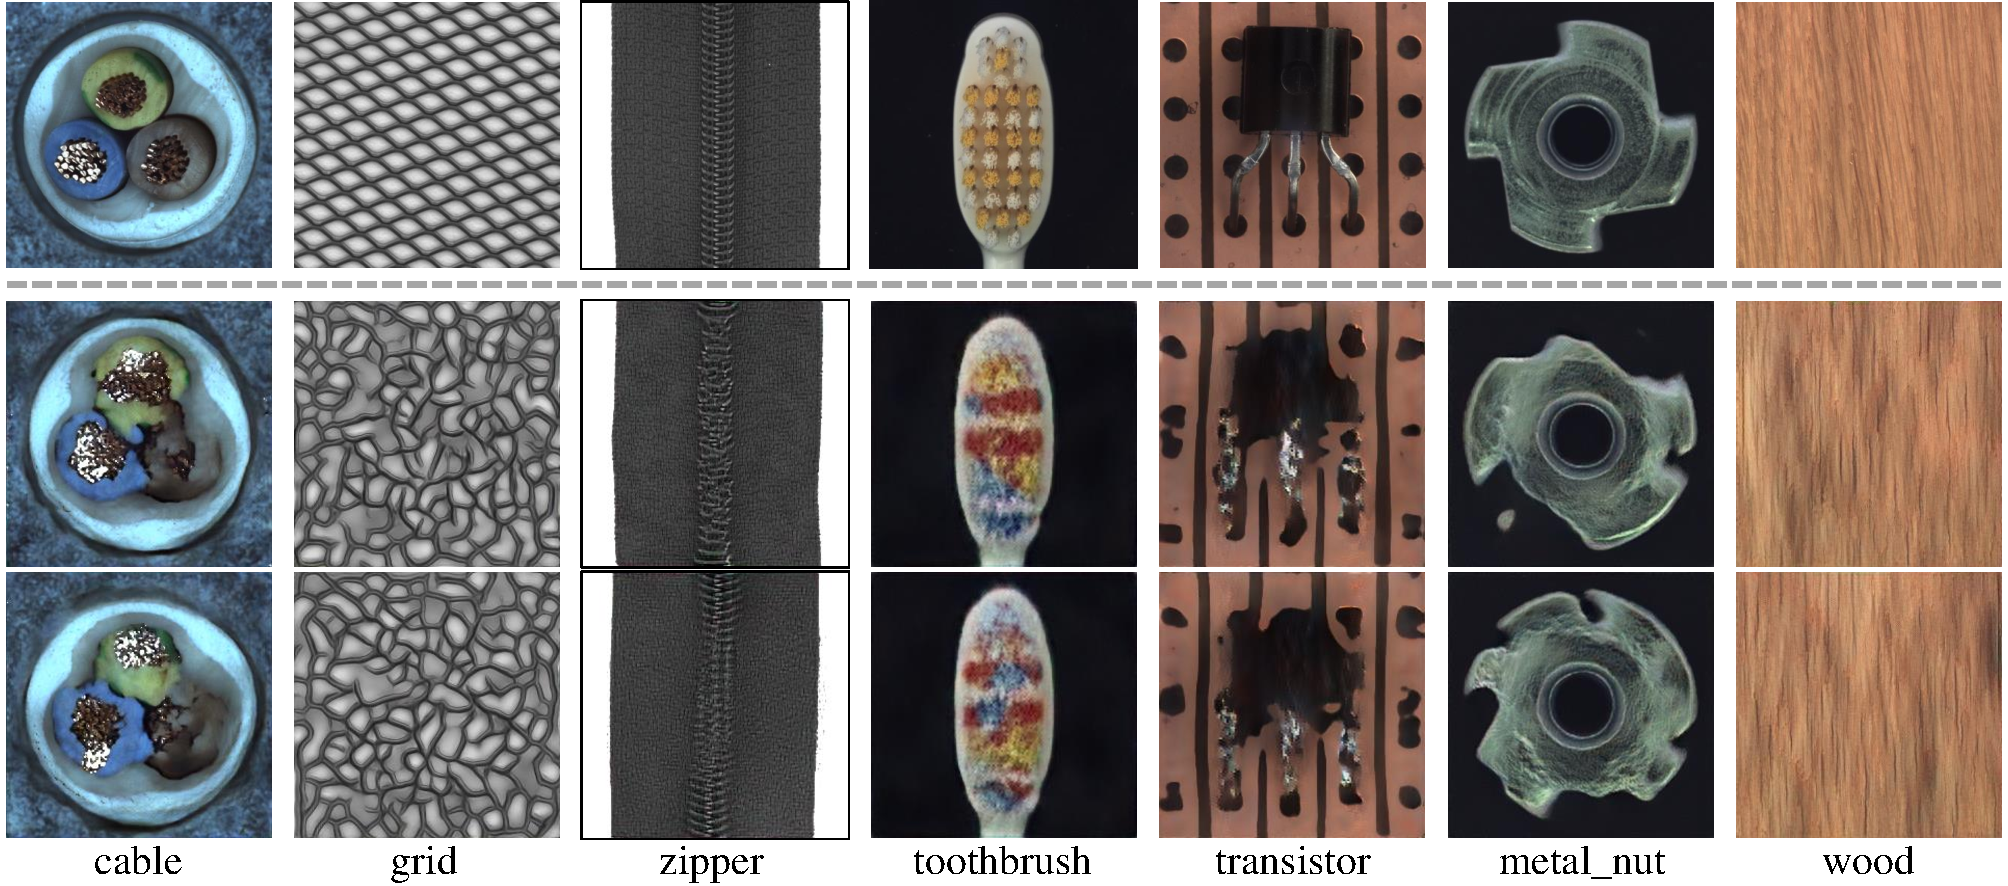
\includegraphics[width=0.7\linewidth]{images/mvtec_generation_results.pdf}
    \caption{Contrastive images generated by level-13 PatchDiff for MVTec AD~\cite{MVTecAD}. } 
    \label{fig: mvtec_generation}
\end{figure*}

\begin{table*}[!h]
    \centering
    % \footnotesize
    % \setlength{\belowcaptionskip}{0.2cm}
    % \setlength{\abovecaptionskip}{0.0cm}
    \renewcommand{\arraystretch}{1.2}
    \resizebox{\textwidth}{!}
    {
\begin{tabular}{cl|c|c|c|c|c|c|c|c}
\toprule
% \multicolumn{2}{c|}{Category} & \makecell[c]{IGD\\\tiny{\citealp{IGD}}} & \makecell[c]{PSVDD\\\tiny{\citealp{PSVDD}}} & \makecell[c]{FCDD\\\tiny{\citealp{FCDD}}} & \makecell[c]{CutPaste\\\tiny{\citealp{CutPaste}}} & \makecell[c]{NSA\\\tiny{\citealp{NSA}}} & \makecell[c]{DRAEM\\\tiny{\citealp{DRAEM}}} & \makecell[c]{DSR\\\tiny{\citealp{DSR}}} & \makecell[c]{GRAD\\\tiny{Ours}} \\ \midrule
\multicolumn{2}{c|}{Category}     & IGD & PSVDD & FCDD & CutPaste &NSA & DRAEM & DSR & GRAD \\ \midrule
\multirow{5}{*}{Texture} 
& carpet & (94.7, 82.8 ) & (92.9, 92.6) & (96.0, - ) & (93.1, 98.3) & (95.5, 95.6) & (95.5,97.0) & (-, \textbf{100.}) & (\textbf{96.5}, 98.2) \\
& grid & (97.7, 97.8 ) & (94.6, 100.) & (91.0, - ) & (\textbf{99.9}, 97.5) & (99.2, 99.9) & (99.7, 99.9) & (-, \textbf{100.}) & (97.2, \textbf{100.}) \\
& leather & (99.5, 95.8) & (90.9, 98.6) & (98.0, - ) & (\textbf{100.}, 99.5) & (99.5, 99.9) & (98.6, \textbf{100.}) & (-, \textbf{100.}) & (98.8, \textbf{100.}) \\
& tile & (78.0, 99.1) & (97.8, 91.4) & (91.0, - ) & (93.4, 90.5) & (\textbf{99.3}, \textbf{100.}) & (99.2, 99.6) & (-, \textbf{100.}) & (95.4, \textbf{100.}) \\
& wood & (89.1, 94.6) & (96.5, 90.8) & (88.0, - ) & (\textbf{98.6}, 95.5) & (90.7, 97.5) & (96.4, \textbf{99.1}) & (-, 96.3) & (87.2, 98.3) \\
\midrule
\multirow{10}{*}{Object} 
& bottle & (92.2, \textbf{100.}) & (98.6, 98.1) & (97.0, - ) & (98.3, 97.6) & (98.3, 97.7) & (\textbf{99.1}, 99.2) & (-, \textbf{100.}) & (96.5, \textbf{100.}) \\
& cable & (84.7, 90.6) & (90.3, 96.8) & (90.0, - ) & (80.6, 90.0) & (96.0, 94.5) & (94.7, 91.8) & (-, 93.8) & (\textbf{98.4}, \textbf{99.3}) \\
& capsule & (\textbf{97.7}, 91.5) & (76.7, 95.8) & (93.0, - ) & (96.2, 97.4) & (97.6, 95.2) & (94.3, \textbf{98.5}) & (-, 98.1) & (97.1, 96.4) \\
& hazelnut & (98.0, 99.7) & (92.0, 97.5) & (95.0, - ) & (97.3, 97.3) & (97.6, 94.7) & (\textbf{99.7}, \textbf{100.}) & (-, 95.6) & (96.6, 98.1) \\
& metal nut & (92.6, 91.3) & (94.0, 98.0) & (94.0, - ) & (99.3, 93.1) & (98.4, 98.7) & (\textbf{99.5}, 98.7) & (-, 98.5) & (93.7, \textbf{100.}) \\
& pill & (97.3, 87.3) & (86.1, 95.1) & (81.0, - ) & (92.4, 95.7) & (\textbf{98.5}, \textbf{99.2}) & (97.6, 98.9) & (-, 97.5) & (98.1, 95.7) \\
& screw & (97.0, 82.5) & (81.3, 95.7) & (86.0, - ) & (86.3, \textbf{96.7}) & (96.5, 90.2) & (97.6, 93.9) & (-, 96.2) & (\textbf{99.2}, 96.0) \\
& toothbrush & (97.7, 99.7) & (\textbf{100.}, 98.1) & (94.0, - ) & (98.3, 98.1) & (94.9, \textbf{100.}) & (98.1, \textbf{100.}) & (-, 99.7) & (98.0, 99.7) \\
& transistor & (84.4, 90.6) & (91.5, 97.0) & (88.0, - ) & (95.5, 93.0) & (88.0, 95.1) & (90.9, 93.1) & (-, 97.8) & (\textbf{97.8}, \textbf{100.}) \\
& zipper & (96.7, 97.0) & (97.9, 95.1) & (92.0, - ) & (\textbf{99.4}, 99.3) & (94.2, 99.8) & (98.9, \textbf{100.}) & (-, \textbf{100.}) & (98.3, 99.7) \\
\midrule
\multicolumn{2}{c|}{Average} & (93.1, 93.4) & (92.5, 93.2 ) & (92.1, 95.7) & (95.2, 96.0) & (96.3, 97.2) & (\textbf{97.3}, 98.0) & (-, 98.2) & (96.8, \textbf{98.7}) \\
\bottomrule
\end{tabular}}
\caption{Anomaly detection performance on MVTec AD dataset~\cite{MVTecAD}. Both pixel-level (left) and image-level (right) AUROC results are shown in each column. The best results are in bold.}
\label{tab: mvtec_main_detail}
\end{table*}

\subsection{Anomaly Detection and Localization}
In the main body, we exclusively present the averaged performance comparison on MVTec AD. In this section, we extend our analysis to provide a detailed result of the anomaly detection and localization performance across each individual sub-dataset within MVTec AD, and display anomaly maps on MVTec AD in Fig.~\ref{fig: main_mvtec_ad_results}. As shown in Table~\ref{tab: mvtec_main_detail}, we compare GRAD to IGD~\cite{IGD}, PSVDD~\cite{PSVDD}, FCDD~\cite{FCDD}, CutPaste~\cite{CutPaste}, NSA~\cite{NSA}, DRAEM~\cite{DRAEM}, and DSR~\cite{DSR}, all of which are independent of pretrained feature extractors. It is easy to find GRAD achieves a strong detection and localization of anomalies.  

\begin{figure*}[!h]
    \centering
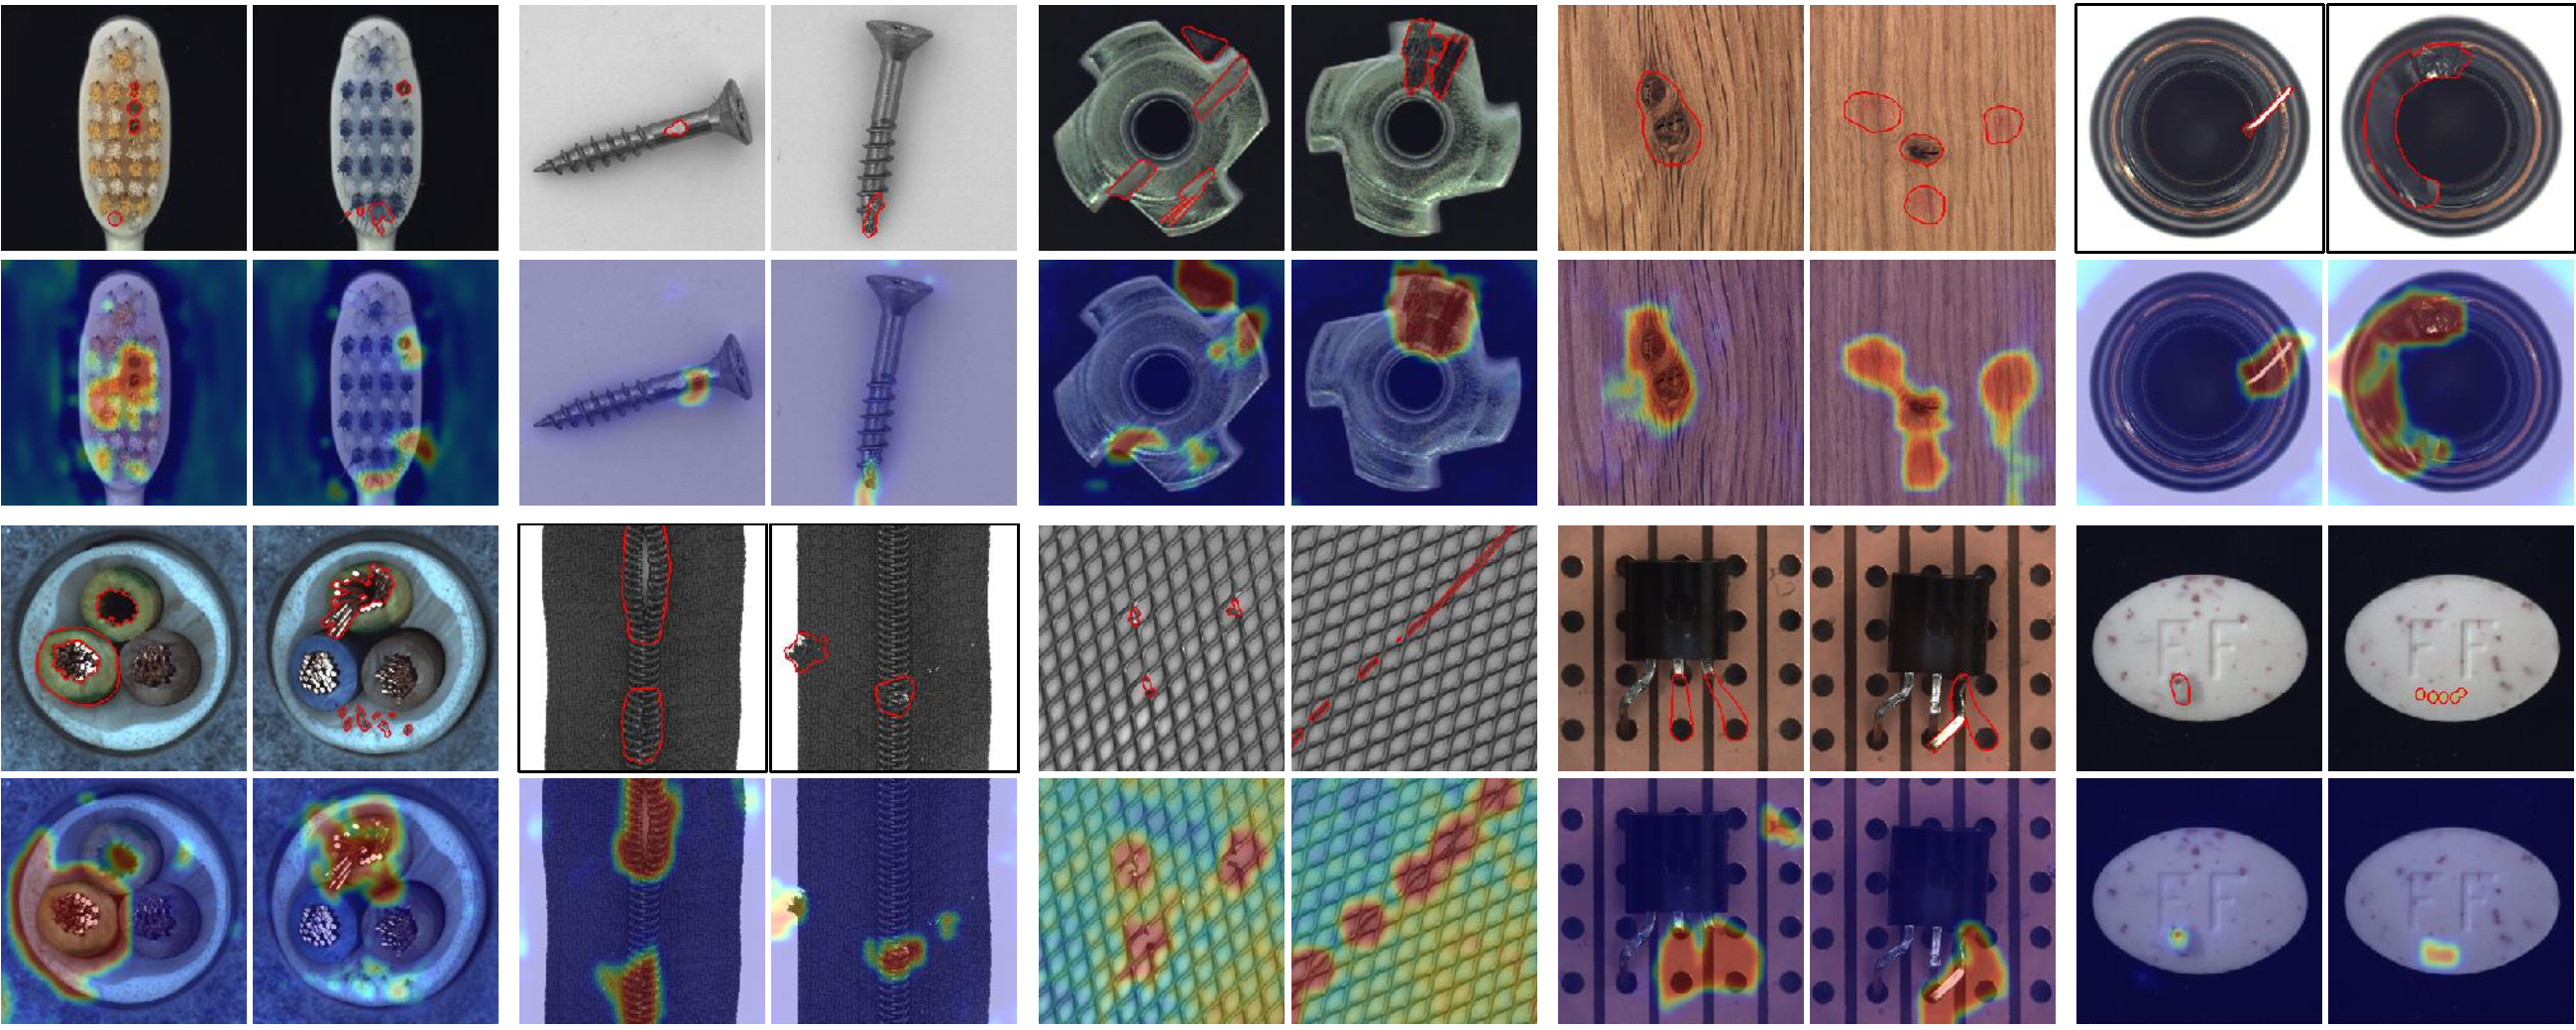
\includegraphics[width=0.9\linewidth]{images/mvtec_results.pdf}
    \caption{Defect localization results of GRAD on MVTec AD~\cite{MVTecAD}. } 
    \label{fig: main_mvtec_ad_results}
    % \vspace{-0.2cm}
\end{figure*}


% In addition, as shown in Table~\ref{tab:ablation_GRad_level}, we conduct an ablations study on selecting levels of patch-level detectors. It is easy to find that when integrating all three different levels of detectors, GRAD can achieve a strong performance for the detection of structural as well as logical anomalies.

% \begin{table}[!htbp]
% \centering
% \footnotesize
% \resizebox{0.3\textwidth}{!}{
% \begin{tabular}{ccc|c}
% \toprule
% \multicolumn{3}{c|}{Level Settings}& Image-level \\
% 136 & 68 & 34  & AUROC\\
% \midrule
% \checkmark &   \ding{55} & \ding{55}   &  85.2   \\
% \ding{55}& \checkmark & \ding{55} & 85.4 \\
% \ding{55}&\ding{55} & \checkmark & 75.1\\
% \checkmark & \checkmark & \ding{55}   &  86.8     \\ %
% \checkmark &   \ding{55} & \checkmark   &  86.4   \\
% \ding{55} & \checkmark & \checkmark  & 86.2 \\
% \checkmark & \checkmark & \checkmark &  \textbf{87.5}  \\
% \bottomrule
% \end{tabular}}
% \caption{Ablation study on detector levels. Detection AUROC results on MVTec LOCO dataset. The best results are in bold.}
% \label{tab:ablation_GRad_level}
% \end{table}



% \bibliography{aaai24}
% \bibliographystyle{aaai24}

% \end{document}


\end{document}
